% ==============================================================================
% 第 18 章：更丰富的数据形态（树） (Chapter 18: More on Forms of Data (Trees))
% ==============================================================================

\chapter{更丰富的数据形态（树）}
\label{sec:ch18_trees}

编程与诗歌有几分相似。正如诗人那样，程序员常常在看似没有现实功用的纯粹构想上磨砺技艺。他们如同上一章所解释的那样，一直在不断地修改与推敲代码。本章将引入日益复杂的数据形态——它们乍看之下似乎脱离了现实世界的具体功用。即使我们为之提供了某种启发性的背景，所选定的数据类别也纯粹到了极致，你在日后的实际开发中或许很难直接原样遇到它们。

然而，本章充分展现了设计配方的全部威力，并向你展示了现实世界程序所必须应对的复杂数据类型。为了将这些内容与你未来作为程序员的职业生涯联系起来，我们为各个小节冠以贴切的名称：树（trees）、森林（forests）与 S-表达式（S-expressions）。这些概念构成了现实世界处理诸如层次结构、文件系统乃至 XML 等复杂数据的理论基石。

\section{树 }
\label{sec:19.1_trees}

我们每个人都有一张家谱（family tree）。绘制家谱的一种直观方式是：每当一个孩子出生时，就添加一个元素，并将其连接到其父亲与母亲的元素上。对于那些父母未知的人，则无需引出连线。这种记录方式被称为\term{祖先家谱}（ancestor family tree），因为对于任意给定的人，树上的指针都指向上溯的所有已知祖先。

图~\ref{fig:111} 展示了一个三代的家谱。Gustav 是 Eva 与 Fred 的孩子，而 Eva 又是 Carl 与 Bettina 的孩子。除人名与亲属关系外，该树还记录了出生年份与眼睛颜色。基于这幅草图，你很容易想象一个延伸多代的庞大家谱，或者记录更多维信息的家谱。

\begin{figure}[htbp]
  \centering
  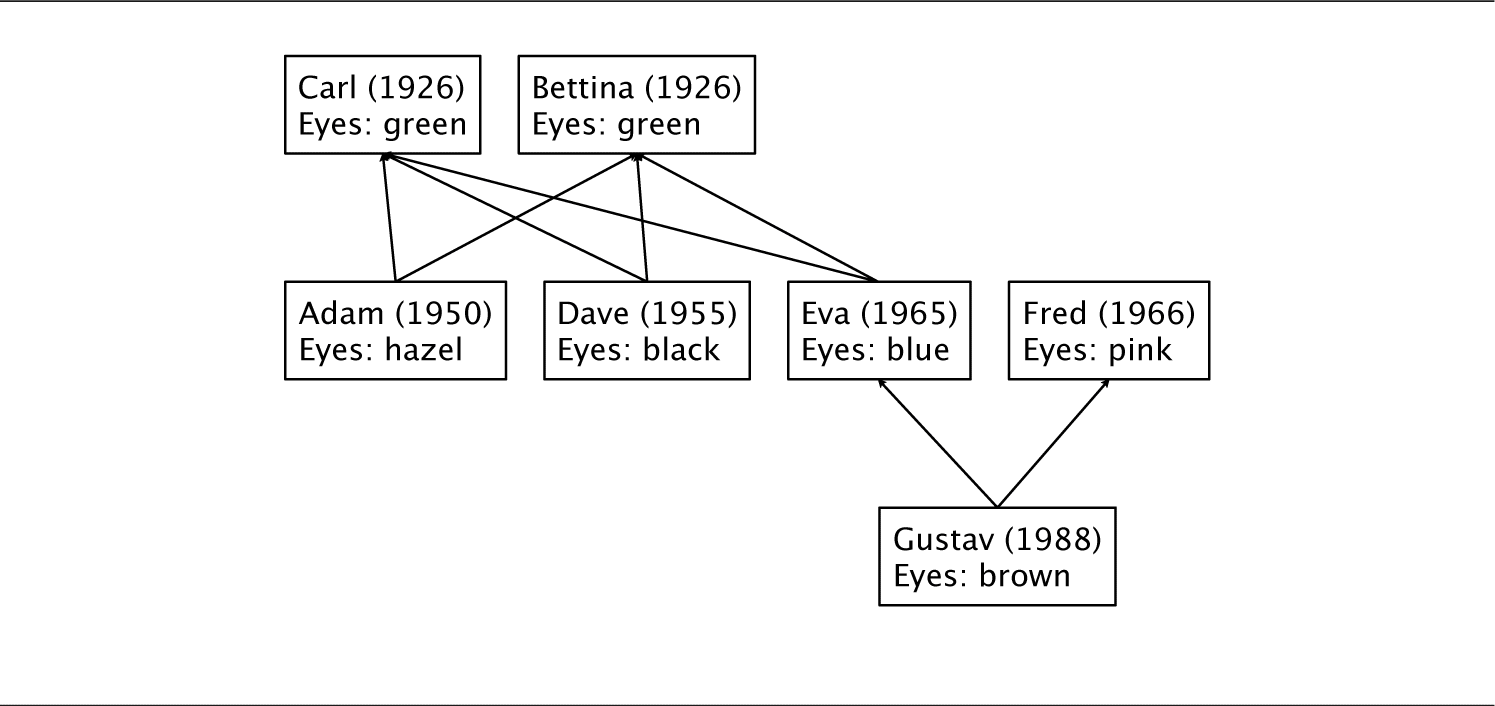
\includegraphics[width=0.85\textwidth]{images/00450.png}
  \caption{家谱图 (A family tree)}
  \label{fig:111}
\end{figure}

一旦家谱规模庞大，将其表示为程序中的数据并设计能够处理此类数据的程序就变得顺理成章。鉴于家谱中的一个节点汇集了五项信息——父亲、母亲、姓名、出生年份以及眼睛颜色——我们应当定义一个结构体类型：

\begin{lstlisting}[language=BSL]
(define-struct child [father mother name date eyes])
\end{lstlisting}

该结构体类型的定义自然引导出一份数据定义：

\begin{lstlisting}[language=BSL]
; Child 是一个结构体：
;   (make-child Child Child String N String)
\end{lstlisting}

虽然这份数据定义看起来非常直观，但它实际上是\textbf{无法使用}的。它引用了自身，然而由于它没有任何基本分支（clause），我们根本无法构造出一个合法的 \code{Child} 实例。简言之，我们必须无休止地写下去：

\begin{lstlisting}[language=BSL]
(make-child (make-child (make-child ...) ...) ...)
\end{lstlisting}

这将陷入无限循环。为了避免这种无意义的数据定义，我们要求\textbf{自引用数据定义必须包含多个分支，且其中至少有一个分支不回引该数据定义自身}。

让我们暂时搁置数据定义的最终定稿，先通过实验来探索。假设我们要向现有的家谱中添加一个孩子，且父母的表示已经存在。在这种情况下，我们只需构建一个新的 \code{child} 结构体。例如，在已经表示了 Carl 与 Bettina 的程序中，要表示 Adam，只需添加如下结构体：

\begin{lstlisting}[language=BSL]
(define Adam
  (make-child Carl Bettina "Adam" 1950 "hazel"))
\end{lstlisting}

这里假定 \code{Carl} 与 \code{Bettina} 代表 Adam 父母的家谱表示。

然而，某个人的父母可能是未知的，就像图~\ref{fig:111} 中 Bettina 的父母那样。即便如此，在 \code{child} 表示中，我们依然必须为相应的父母字段填充值。无论我们选择什么数据，它都必须明确表达\textbf{信息的缺失}。一方面，我们可以从现有值池中选用 \code{\#false}、\code{"none"} 或 \code{'()}；另一方面，我们更应当明确宣称：该信息在当前家谱中不存在。通过引入一个命名恰当的结构体类型，可以最优雅地达成这一目标：

\begin{lstlisting}[language=BSL]
(define-struct no-parent [])
\end{lstlisting}

现在，为了为 Bettina 构建一个 \code{child} 结构体，我们可以这样写：

\begin{lstlisting}[language=BSL]
(make-child (make-no-parent) (make-no-parent) "Bettina" 1926 "green")
\end{lstlisting}

当然，如果只有一方父母信息缺失，我们就只需在对应字段中填入这一特殊值。

上述实验为我们带来了两点深刻见解：
\begin{enumerate}
  \item 我们寻求的不是一个描述如何生成单个 \code{child} 结构体实例的数据定义，而是一个描述\textbf{如何表示完整家谱}的数据定义。
  \item 该数据定义包含两个分支：一个分支描述未知的家谱，另一个分支描述已知的家谱。
\end{enumerate}

\begin{lstlisting}[language=BSL]
(define-struct no-parent [])
(define-struct child [father mother name date eyes])

; 一个 FT（Family Tree，家谱）是下列之一：
; -- (make-no-parent)
; -- (make-child FT FT String N String)
\end{lstlisting}

由于表示“无父母”的树在程序中频繁出现，我们定义 \code{NP} 作为简写，并略微修饰数据定义：

\begin{lstlisting}[language=BSL]
(define NP (make-no-parent))

; 一个 FT 是下列之一：
; -- NP
; -- (make-child FT FT String N String)
\end{lstlisting}

遵循第 9 章的设计配方，我们利用数据定义来创建家谱的数据样例。具体而言，我们将图~\ref{fig:111} 中的家谱翻译为数据表示。Carl 的信息很容易翻译：

\begin{lstlisting}[language=BSL]
(make-child NP NP "Carl" 1926 "green")
\end{lstlisting}

Bettina 和 Fred 也用类似的 \code{child} 实例表示。而 Adam 则需要嵌套子节点，分别对应 Carl 和 Bettina：

\begin{lstlisting}[language=BSL]
(make-child (make-child NP NP "Carl" 1926 "green")
            (make-child NP NP "Bettina" 1926 "green")
            "Adam"
            1950
            "hazel")
\end{lstlisting}

由于 Carl 和 Bettina 的记录在构建 Dave 和 Eva 时也需要用到，更好的做法是引入变量定义来命名特定的 \code{child} 实例，并在其他地方引用这些变量名。图~\ref{fig:112} 展示了图~\ref{fig:111} 完整家谱的数据表示。请仔细观察这棵树，它将作为后续设计练习的持续案例。

\begin{figure}[htbp]
  \centering
  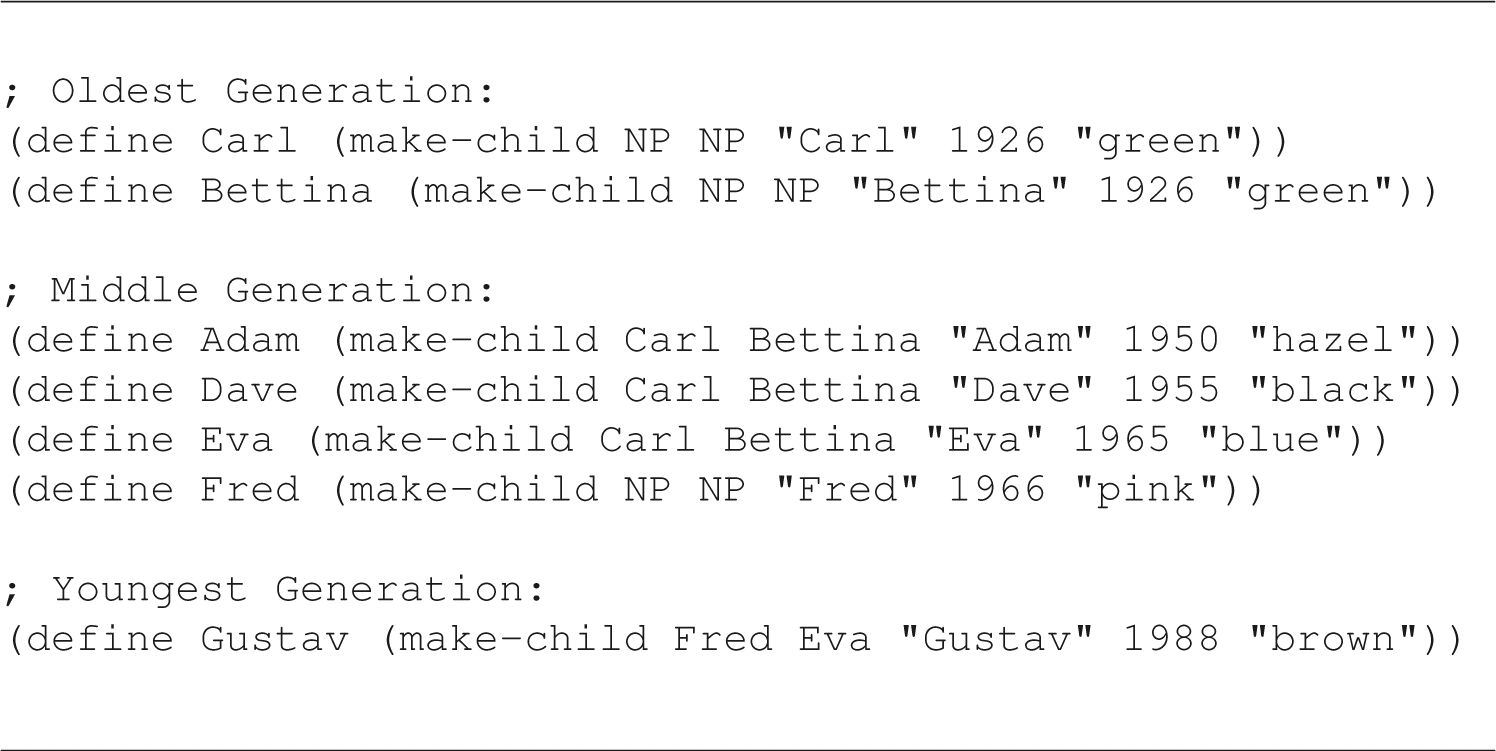
\includegraphics[width=0.85\textwidth]{images/00453.png}
  \caption{样本家谱的数据表示 (A data representation of the sample family tree)}
  \label{fig:112}
\end{figure}

在设计具体的家谱处理函数之前，我们先来看看此类函数的通用组织结构。换句话说，在尚未确定具体任务的情况下，尽可能推进设计配方的步骤。我们从设计配方的第二步（签名、目的说明与函数头）开始：

\begin{lstlisting}[language=BSL]
; FT -> ???
; ...
(define (fun-FT an-ftree)
  ...)
\end{lstlisting}

虽然我们尚未陈述函数的具体目的，但已知它接收一个家谱作为主要输入。签名中的 \code{???} 表明输出类型未定，省略号则提醒我们目的尚待明确。

缺乏具体目的意味着我们无法编写具体的功能示例。然而，我们完全可以依据 \code{FT} 的数据定义结构来设计模板。由于 \code{FT} 包含两个分支，模板必须包含一个含有两个条件分支的 \code{cond} 表达式：

\begin{lstlisting}[language=BSL]
(define (fun-FT an-ftree)
  (cond
    [(no-parent? an-ftree) ...]
    [(child? an-ftree) ...]))
\end{lstlisting}

当输入满足 \code{no-parent?} 时，该结构不包含任何附加数据，因此第一个分支处理完毕。对于第二个分支，输入包含五项数据，我们在模板中用五个选择器表达式标明：

\begin{lstlisting}[language=BSL]
(define (fun-FT an-ftree)
  (cond
    [(no-parent? an-ftree) ...]
    [else
     (... (child-father an-ftree) ...
      ... (child-mother an-ftree) ...
      ... (child-name an-ftree) ...
      ... (child-date an-ftree) ...
      ... (child-eyes an-ftree) ...)]))
\end{lstlisting}

模板构造的最后一步涉及\textbf{自引用}。如果数据定义引用了自身，函数极有可能发生递归，模板通过启发性的自然递归调用体现这一点。\code{FT} 的定义包含两处自引用（父亲与母亲字段均是 \code{FT}），因此模板需要两处自然递归：

\begin{lstlisting}[language=BSL]
(define (fun-FT an-ftree)
  (cond
    [(no-parent? an-ftree) ...]
    [else
     (... (fun-FT (child-father an-ftree)) ...
      ... (fun-FT (child-mother an-ftree)) ...
      ... (child-name an-ftree) ...
      ... (child-date an-ftree) ...
      ... (child-eyes an-ftree) ...)]))
\end{lstlisting}

具体来说，在第二个 \code{cond} 分支中，\code{fun-FT} 分别作用于父亲与母亲的数据表示，因为数据定义的第二个分支恰恰包含了这两处对 \code{FT} 的自引用。

现在让我们转向一个具体问题：设计 \code{blue-eyed-child?} 函数。该函数的目的是确定给定家谱中是否存在眼睛颜色为蓝色的孩子。我们可以复制、粘贴并重命名 \code{fun-FT} 来获得模板，将 \code{???} 替换为 \code{Boolean} 并添加目的说明：

\begin{lstlisting}[language=BSL]
; FT -> Boolean
; 判断给定家谱中是否包含蓝眼睛的孩子
(define (blue-eyed-child? an-ftree)
  (cond
    [(no-parent? an-ftree) ...]
    [else
     (... (blue-eyed-child? (child-father an-ftree)) ...
      ... (blue-eyed-child? (child-mother an-ftree)) ...
      ... (child-name an-ftree) ...
      ... (child-date an-ftree) ...
      ... (child-eyes an-ftree) ...)]))
\end{lstlisting}

根据设计配方，我们回溯到用例设计步骤。如果以 Carl 开始，Carl 的眼睛是 \code{"green"}，其祖先树均为空，因此 Carl 的家谱中绝不可能有蓝眼睛的孩子：

\begin{lstlisting}[language=BSL]
(check-expect (blue-eyed-child? Carl) #false)
\end{lstlisting}

相反，Gustav 的母亲 Eva 拥有蓝眼睛：

\begin{lstlisting}[language=BSL]
(check-expect (blue-eyed-child? Gustav) #true)
\end{lstlisting}

现在我们准备填充函数体。函数区分两种情形：\code{no-parent} 和 \code{child}。对于第一种情形，家谱为空，自然不可能包含蓝眼睛的孩子，因此结果为 \code{\#false}。

对于第二种情形，依据设计配方，我们首先明确模板中各个表达式的作用：
\begin{enumerate}
  \item \code{(blue-eyed-child? (child-father an-ftree))} 判断父亲一方的家谱中是否有蓝眼睛的孩子；
  \item \code{(blue-eyed-child? (child-mother an-ftree))} 判断母亲一方的家谱中是否有蓝眼睛的孩子；
  \item 选择器表达式 \code{(child-name an-ftree)}、\code{(child-date an-ftree)} 和 \code{(child-eyes an-ftree)} 分别提取当前孩子的姓名、出生年份和眼睛颜色。
\end{enumerate}

显然，如果当前孩子的眼睛字段为 \code{"blue"}，函数直接返回 \code{\#true}。姓名和出生年份对于判断眼睛颜色无用。剩下的问题是如何组合这三个布尔表达式：如果当前孩子是蓝眼睛，或者父亲一方有蓝眼睛，或者母亲一方有蓝眼睛，则整棵家谱中就存在蓝眼睛：

\begin{lstlisting}[language=BSL]
(or (string=? (child-eyes an-ftree) "blue")
    (blue-eyed-child? (child-father an-ftree))
    (blue-eyed-child? (child-mother an-ftree)))
\end{lstlisting}

图~\ref{fig:113} 给出了完整的函数定义。

\begin{figure}[htbp]
  \centering
  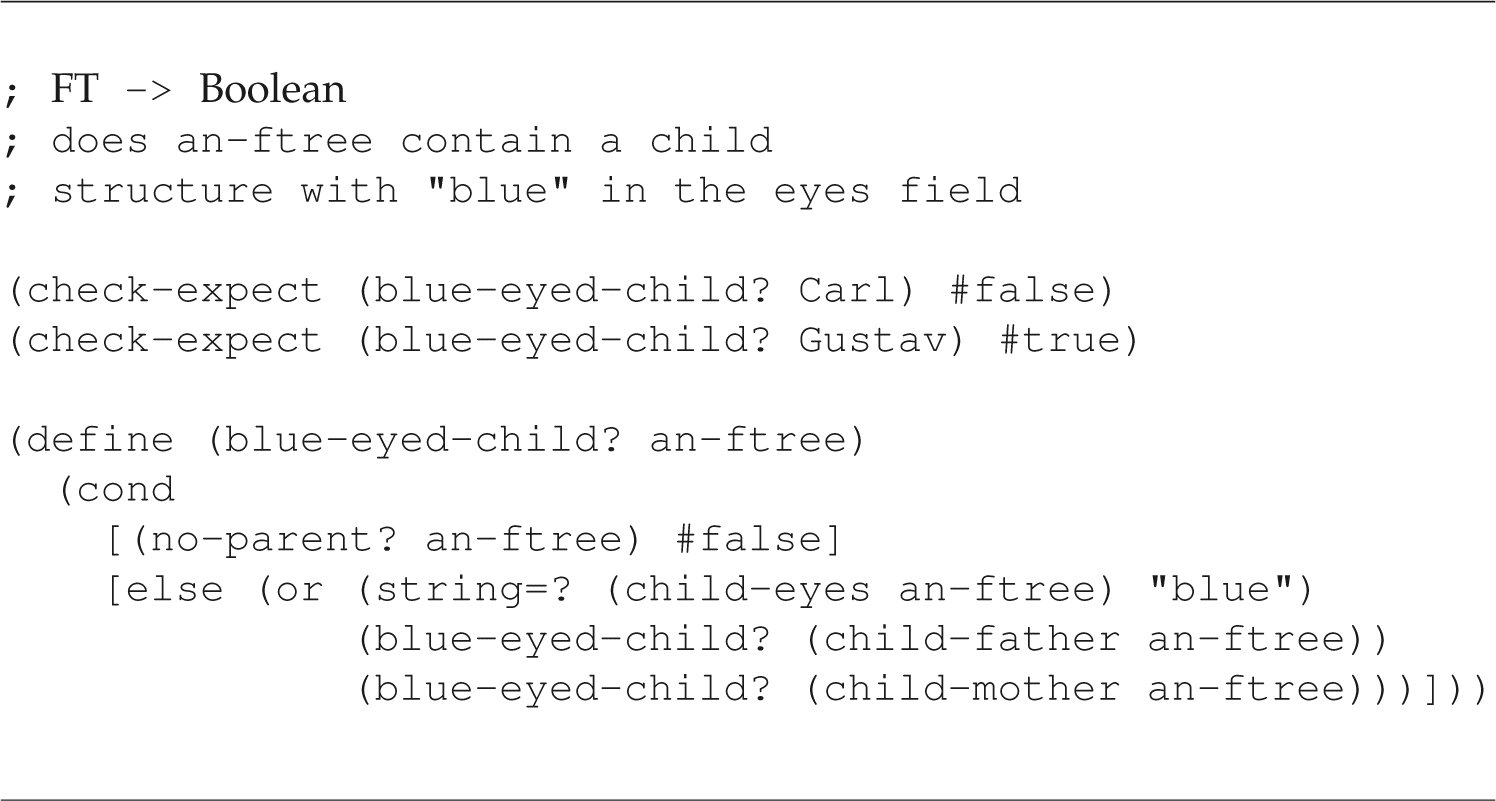
\includegraphics[width=0.85\textwidth]{images/00458.png}
  \caption{在祖先树中寻找蓝眼睛的孩子 (Finding a blue-eyed child in an ancestor tree)}
  \label{fig:113}
\end{figure}

由于这是本书中第一个使用双重递归调用的函数，图~\ref{fig:114} 模拟了单步求值器对 \code{(blue-eyed-child? Carl)} 的求值轨迹，帮助你体会树形递归的运作机制。

\begin{figure}[htbp]
  \centering
  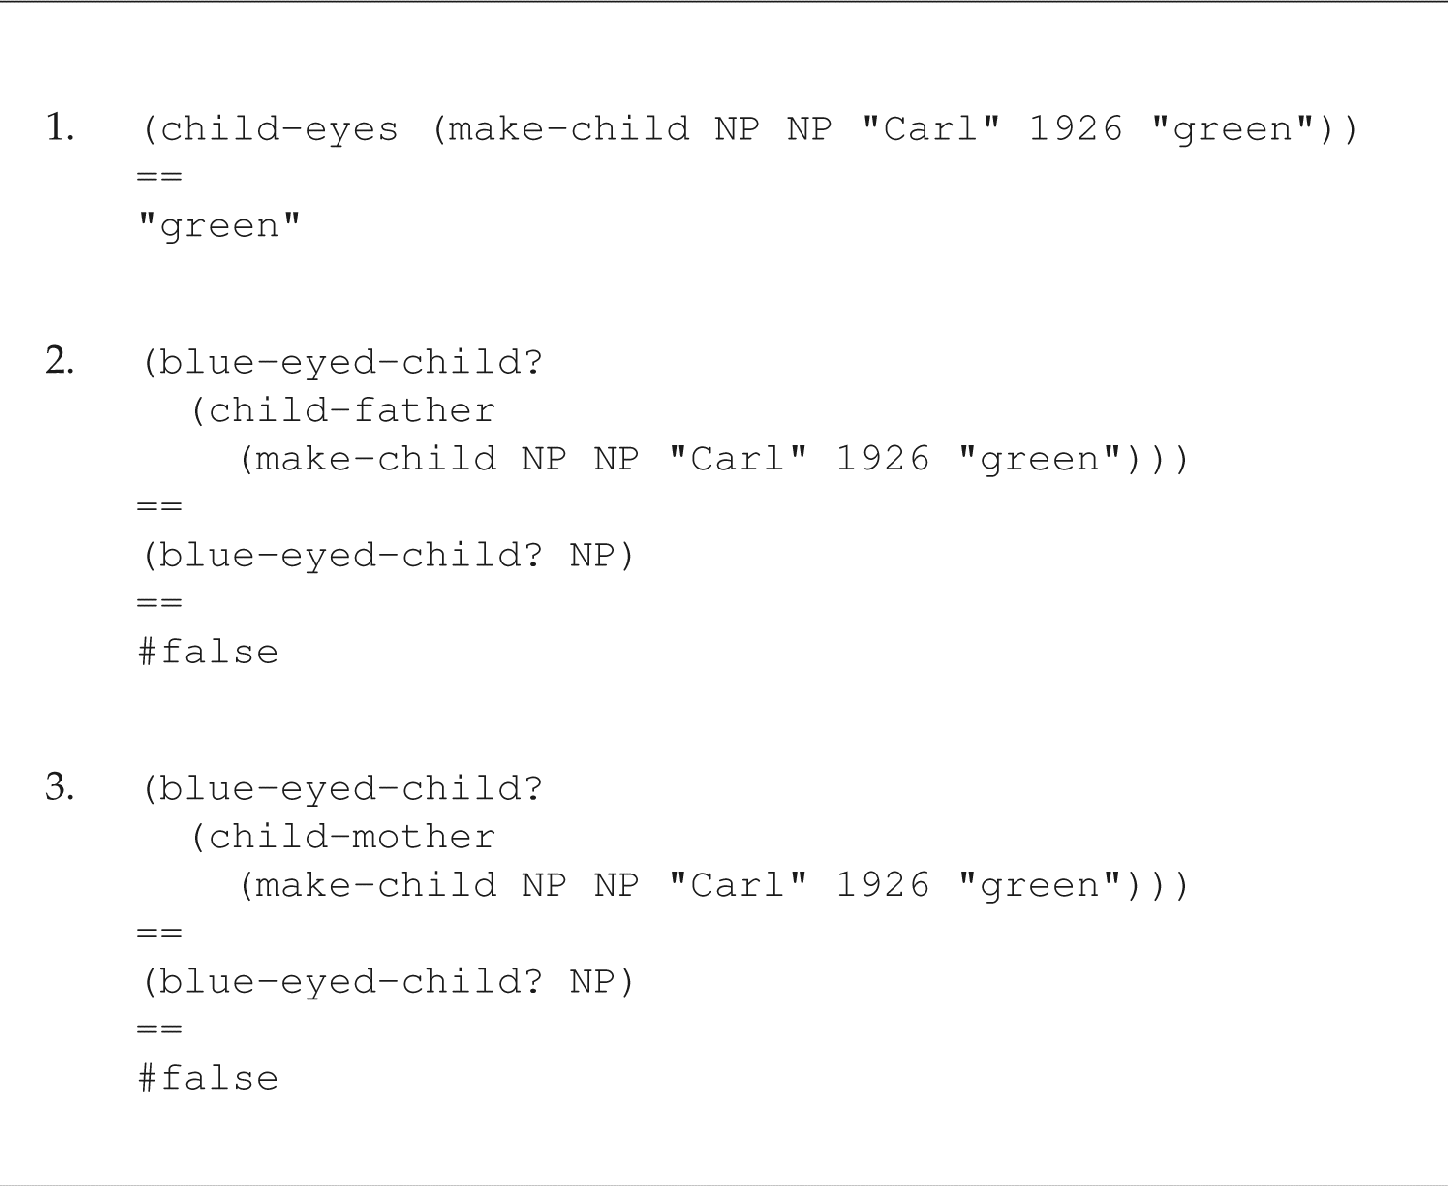
\includegraphics[width=0.85\textwidth]{images/00461.png}
  \caption{树结构的求值推导计算 (Calculating with trees)}
  \label{fig:114}
\end{figure}

\begin{exercise}{统计家谱中的人数}{310}
开发函数 \code{count-persons}。该函数接收一棵家谱 \code{FT}，统计树中包含的 \code{child} 结构体的总数。
\end{exercise}

\begin{exercise}{计算家谱中的平均年龄}{311}
开发函数 \code{average-age}。该函数接收一棵家谱与当前年份，计算家谱中所有 \code{child} 结构体所代表人物的平均年龄。
\end{exercise}

\begin{exercise}{收集家谱中的眼睛颜色}{312}
开发函数 \code{eye-colors}。该函数接收一棵家谱，生成该树中出现的所有眼睛颜色的列表。某种眼睛颜色在结果列表中可多次出现。\emph{提示：} 使用 \code{append} 拼接递归调用返回的列表。
\end{exercise}

\begin{exercise}{寻找蓝眼睛祖先}{313}
假设我们需要函数 \code{blue-eyed-ancestor?}。它与 \code{blue-eyed-child?} 类似，但仅当给定孩子的\textbf{真正祖先}（即不包含该孩子本人）拥有蓝眼睛时才返回 \code{\#true}。

请首先为该函数编写签名与目的说明：
\begin{lstlisting}[language=BSL]
; FT -> Boolean
(define (blue-eyed-ancestor? an-ftree)
  ...)
\end{lstlisting}

为了理解其区别，以 Eva 为例：Eva 本人是蓝眼睛，但她没有蓝眼睛的祖先：
\begin{lstlisting}[language=BSL]
(check-expect (blue-eyed-child? Eva) #true)
(check-expect (blue-eyed-ancestor? Eva) #false)
\end{lstlisting}
而 Gustav 是 Eva 的儿子，他确实拥有蓝眼睛祖先：
\begin{lstlisting}[language=BSL]
(check-expect (blue-eyed-ancestor? Gustav) #true)
\end{lstlisting}

现在假设一位朋友提出了如下解法：
\begin{lstlisting}[language=BSL]
(define (blue-eyed-ancestor? an-ftree)
  (cond
    [(no-parent? an-ftree) #false]
    [else
     (or (blue-eyed-ancestor? (child-father an-ftree))
         (blue-eyed-ancestor? (child-mother an-ftree)))]))
\end{lstlisting}
解释为什么该函数无法通过测试。无论传入什么家谱，该函数的返回值都是什么？你能修复这位朋友的解法吗？
\end{exercise}

\section{森林 }
\label{sec:19.2_forests}

从家谱走向“家庭森林”（Family Forest，简称森林）仅有一步之遥：

\begin{lstlisting}[language=BSL]
; 一个 FF（family forest，家族森林）是下列之一：
; -- '()
; -- (cons FT FF)
; 解释：家族森林表示若干个家族（例如一个城镇中的居民）及其祖先树
\end{lstlisting}

以下是从图~\ref{fig:111} 中摘取的若干树构成的森林示例：

\begin{lstlisting}[language=BSL]
(define ff1 (list Carl Bettina))
(define ff2 (list Fred Eva))
(define ff3 (list Fred Eva Carl))
\end{lstlisting}

前两个森林包含互不相关的家族，第三个则说明：与自然界的森林不同，家族森林中的树木在逻辑上是可以相互重叠的。

现在考虑如下典型问题：

\begin{notebox}[样本问题]
设计函数 \code{blue-eyed-child-in-forest?}，判断给定的家族森林中是否包含眼睛为 \code{"blue"} 的孩子。
\end{notebox}

图~\ref{fig:115} 展示了该问题的直观解法。森林本质上是一个列表，因此可以沿用列表模板。如果列表的每一项都是带有眼睛字段的单一结构体，函数只需遍历这些结构体并进行比较。而在本例中，列表的每一项都是一棵完整的家谱树，幸运的是，我们已经掌握了如何处理家谱树（直接复用 \code{blue-eyed-child?}）。

\begin{figure}[htbp]
  \centering
  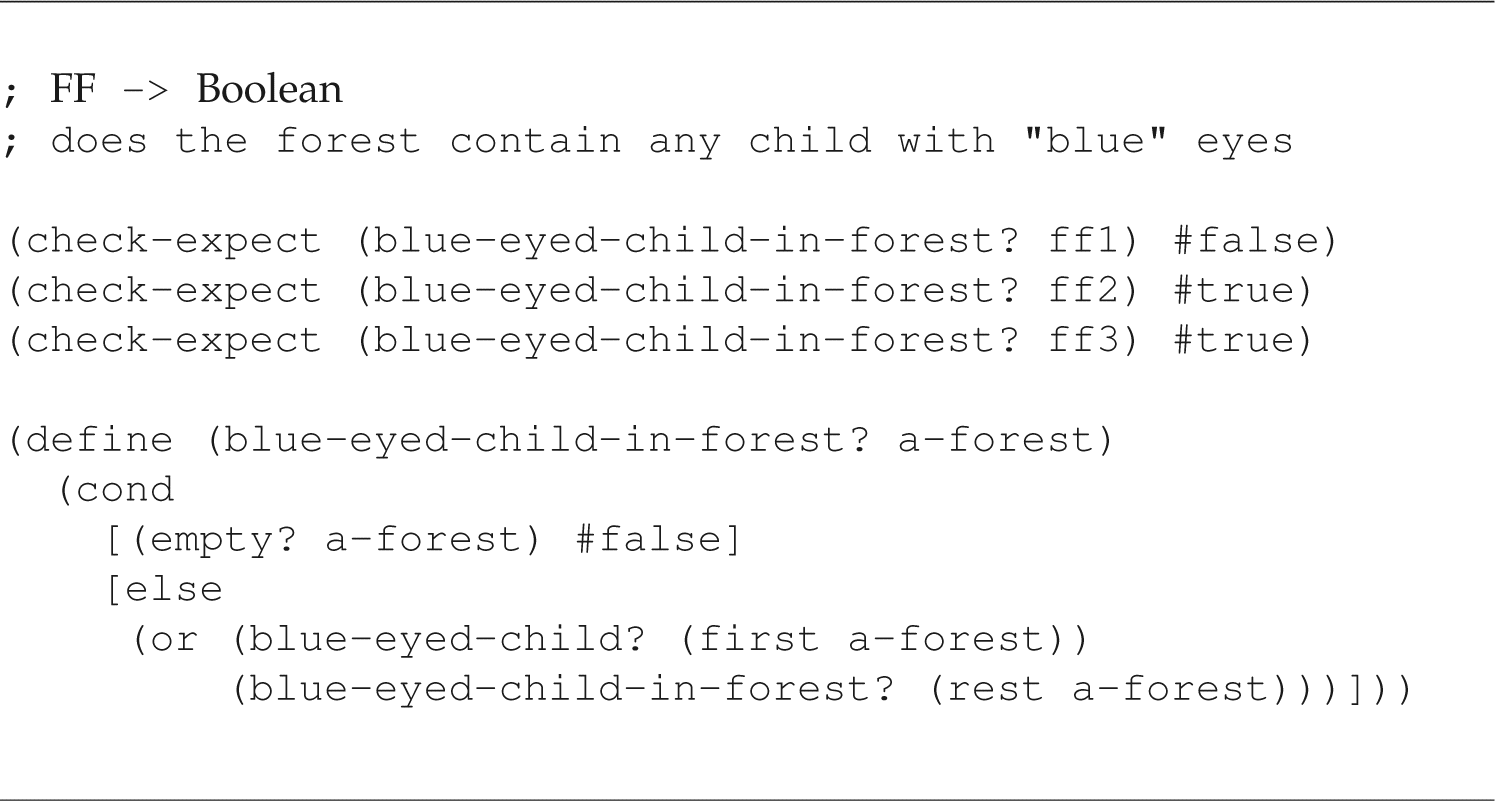
\includegraphics[width=0.85\textwidth]{images/00463.png}
  \caption{在家族森林中寻找蓝眼睛的孩子 (Finding a blue-eyed child in a family forest)}
  \label{fig:115}
\end{figure}

退一步审视图~\ref{fig:115} 的构成。起点是一对数据定义，其中第二个定义引用了第一个，且两者各自包含自引用。结果是一对相互配合的函数定义：第二个函数调用了第一个，且两者各自递归。换句话说，\textbf{函数定义之间的相互引用关系完全镜像了数据定义之间的相互引用关系}。早先章节对这种关系略有涉及，但现在这种结构已足够丰富，值得给予充分的关注。

\begin{exercise}{使用 List-of 抽象重构森林定义}{314}
使用 \code{List-of} 抽象重新表述 \code{FF} 的数据定义。然后对 \code{blue-eyed-child-in-forest?} 做同样的重构。最后，使用前一章学过的列表抽象函数（例如 \code{ormap}）来重新定义 \code{blue-eyed-child-in-forest?}。
\end{exercise}

\begin{exercise}{计算森林中人员的平均年龄}{315}
设计函数 \code{average-age}。该函数接收一个家族森林与一个年份（\code{N}），计算森林中所有 \code{child} 实例的平均年龄。
\emph{注意：} 如果森林中的树存在重叠，直接求和可能导致某些人被重复计算；在本练习中，暂且假设森林中的各棵树互不重叠。
\end{exercise}

\section{S-表达式 }
\label{sec:19.3_sexpr}

虽然插曲 2 非正式地介绍了 S-表达式（S-expression），但我们可以通过三个互相交织的数据定义精确描述它们：

\begin{lstlisting}[language=BSL]
; 一个 S-expr（S-表达式）是下列之一：
; -- Atom
; -- SL

; 一个 SL（S-表达式列表）是下列之一：
; -- '()
; -- (cons S-expr SL)

; 一个 Atom（原子）是下列之一：
; -- Number
; -- String
; -- Symbol
\end{lstlisting}

请回忆：符号（Symbol）在书写时形如单引号开头的字符串，末尾不加引号，例如 \code{'hello}。

S-表达式的思想源自约翰·麦卡锡（John McCarthy）及其 Lisp 团队，他们在 1958 年发明了 S-表达式，以便能够\textbf{用 Lisp 程序来处理 Lisp 程序}。这种看似循环的构想听起来十分玄妙，但正如插曲 2 所述，S-表达式是一种极具通用性的数据形态，屡屡被后人重新发现，最近的大规模应用便是万维网（XML/HTML 与 JSON）。掌握 S-表达式将为我们设计高度交织的数据定义及其处理函数打下坚实基础。

\begin{exercise}{定义 atom? 谓词}{316}
在 BSL 中定义 \code{atom?} 谓词函数，判断给定值是否属于 \code{Atom}。
\end{exercise}

在此之前，本书中尚未出现过像 S-表达式这样复杂的数据定义。然而，只要遵循扩展后的设计配方，你完全能够设计出处理 S-表达式的函数。我们通过一个具体问题来展示这一点：

\begin{notebox}[样本问题]
设计函数 \code{count}，统计某个给定符号在某 S-表达式中出现的总次数。
\end{notebox}

第一步是创建数据样例。S-表达式的定义指出每个 \code{Atom} 都是 \code{S-expr}：
\begin{lstlisting}[language=BSL]
'hello
20.12
"world"
\end{lstlisting}

同样，每个 \code{SL} 既是一个列表，也是一个 \code{S-expr}：
\begin{lstlisting}[language=BSL]
'()
(cons 'hello (cons 20.12 (cons "world" '())))
(cons (cons 'hello (cons 20.12 (cons "world" '()))) '())
\end{lstlisting}

借助插曲 2 的引用（quote）机制，书写 S-表达式变得极为便捷。我们在 DrRacket 交互区中验证这些例子：

\begin{replbox}
> '()
'()
> '(hello 20.12 "world")
(list 'hello #i20.12 "world")
> '((hello 20.12 "world"))
(list (list 'hello #i20.12 "world"))
\end{replbox}

借助 \code{quote}，我们还可以轻松构造形如代码或数据表格的复杂表达式：

\begin{replbox}
> '(define (f x) (+ x 10))
(list 'define (list 'f 'x) (list '+ 'x 10))
> '((mercury 1) (venus 2) (earth 3))
(list (list 'mercury 1) (list 'venus 2) (list 'earth 3))
> '(wing (wing body wing) wing)
(list 'wing (list 'wing 'body 'wing) 'wing)
\end{replbox}

现在为 \code{count} 写出函数头与功能示例：

\begin{lstlisting}[language=BSL]
; S-expr Symbol -> N
; 统计 sy 在 sexp 中出现的总次数
(check-expect (count 'world 'hello) 0)
(check-expect (count '(world hello) 'hello) 1)
(check-expect (count '(((world) hello) hello) 'hello) 2)

(define (count sexp sy)
  0)
\end{lstlisting}

在模板设计阶段，面对相互交织的数据定义，我们需要核心设计准则：

\begin{notebox}[交织数据模板准则]
对于互相交织的数据定义，\textbf{为每个数据定义各创建一个模板}。并行创建它们，并确保模板之间的调用关系与数据定义之间的引用关系完全对应。
\end{notebox}

对于当前问题，我们需要三个模板：
\begin{enumerate}
  \item \code{count}：处理 \code{S-expr}；
  \item \code{count-sl}：处理 \code{SL}；
  \item \code{count-atom}：处理 \code{Atom}。
\end{enumerate}

图~\ref{fig:116} 给出了这三个完整的函数模板。模板之间的调用箭头精确复刻了数据定义之间的引用箭头。

\begin{figure}[htbp]
  \centering
  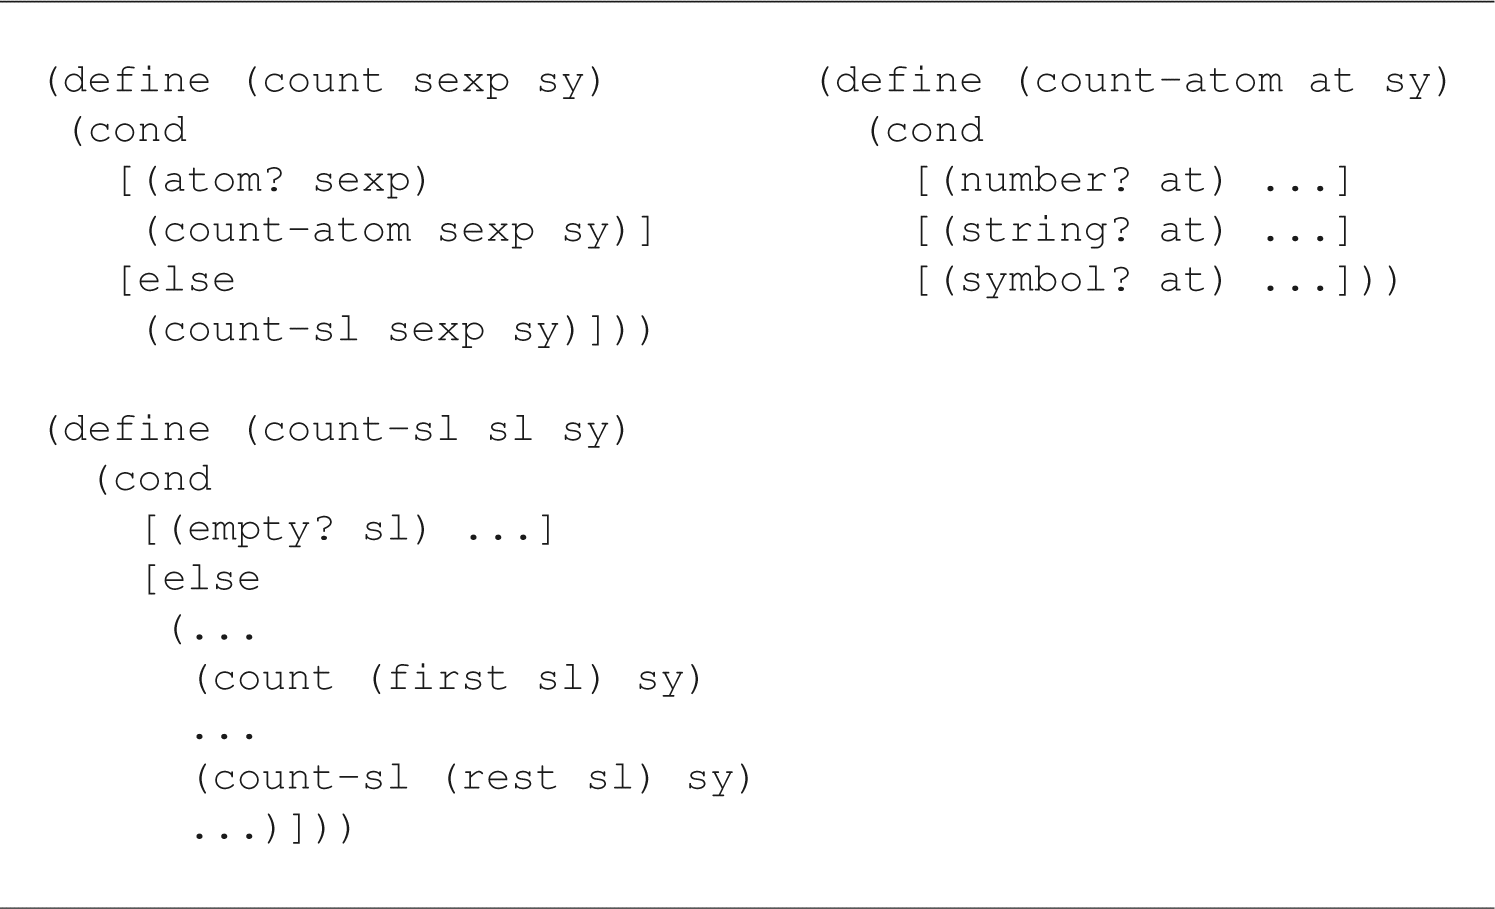
\includegraphics[width=0.85\textwidth]{images/00470.png}
  \caption{S-表达式的处理模板 (A template for S-expressions)}
  \label{fig:116}
\end{figure}

在这些模板的基础上填补空白，便得到了图~\ref{fig:117} 中的完整程序。

\begin{figure}[htbp]
  \centering
  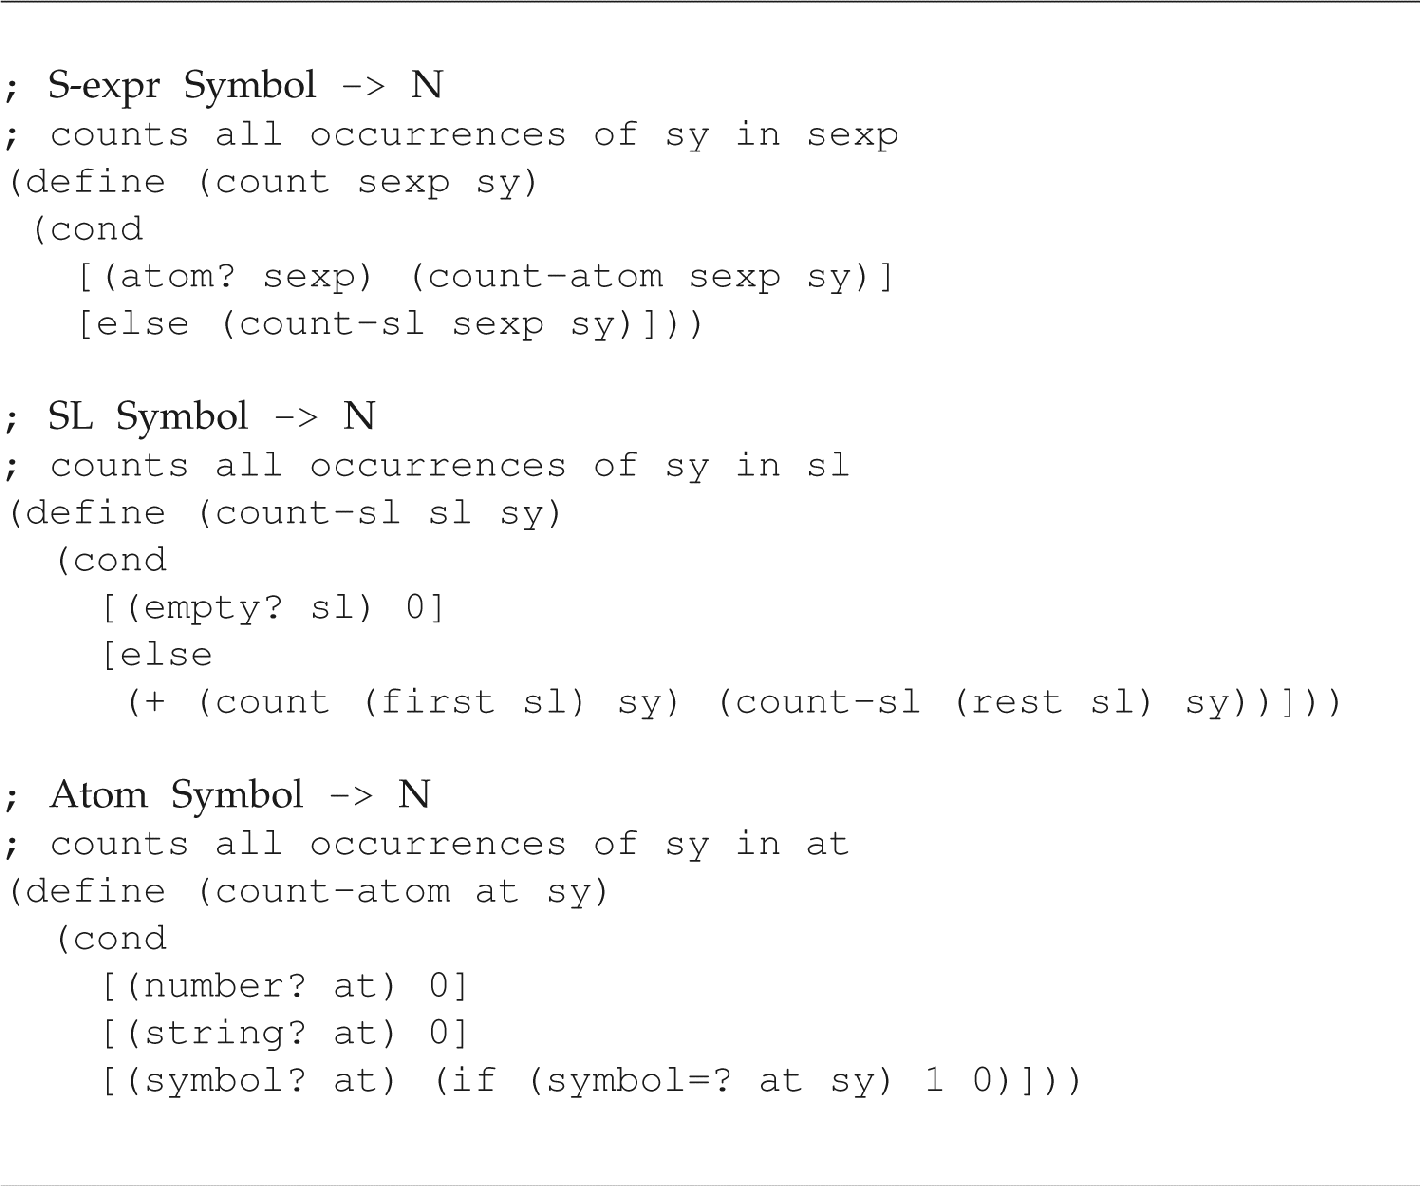
\includegraphics[width=0.85\textwidth]{images/00471.png}
  \caption{S-表达式的计数程序 (A program for S-expressions)}
  \label{fig:117}
\end{figure}

让我们逐一审视各个关键分支：
\begin{itemize}
  \item \code{[(atom? sexp) (count-atom sexp sy)]}：若 \code{sexp} 是原子，则转交专职函数 \code{count-atom} 处理；
  \item \code{[else (+ (count (first sl) sy) (count-sl (rest sl) sy))]}：列表由第一项（一个 \code{S-expr}）和其余项（一个 \code{SL}）组成，分别调用对应函数统计后相加；
  \item \code{[(symbol? at) (if (symbol=? at sy) 1 0)]}：若原子是符号且与目标符号相等，则计数为 1，否则为 0。
\end{itemize}

\begin{exercise}{使用 local 整合多函数}{317}
由三个互相关联的函数组成的程序，理应使用 \code{local} 表达式体现这种从属关系。

请将图~\ref{fig:117} 中的程序重组为包含内部辅助函数的单个 \code{count} 函数。由于第二个参数 \code{sy} 在整个遍历过程中从不改变，你可以从局部辅助函数的参数列表中移除它，从而向读者表明 \code{sy} 是遍历过程中的全局常量。
\end{exercise}

\begin{exercise}{计算 S-表达式的深度}{318}
设计函数 \code{depth}。该函数接收一个 S-表达式并计算其嵌套深度。\code{Atom} 的深度为 1。S-表达式列表的深度为其各元素深度的最大值加 1。空列表的深度可视为 0 或 1（请明确你的约定）。
\end{exercise}

\begin{exercise}{S-表达式的符号替换}{319}
设计函数 \code{substitute}。它接收一个 S-表达式 \code{s} 以及两个符号 \code{old} 和 \code{new}。其结果与 \code{s} 相同，只是其中所有出现的 \code{old} 均被替换为 \code{new}。
\end{exercise}

\begin{exercise}{重构并化简 S-expr 定义}{320}
重新表述 \code{S-expr} 的数据定义，将第一个分支直接展开为 \code{Atom} 的三个分支，并在第二个分支中使用 \code{[List-of S-expr]} 抽象。针对这一新定义重新设计 \code{count} 函数。你能否结合 \code{lambda} 进一步化简该函数？
\end{exercise}

\begin{exercise}{对 S-表达式中的原子进行抽象}{321}
对 \code{S-expr} 和 \code{SL} 的数据定义进行参数化抽象，使其能够容纳不同种类的原子数据。
\end{exercise}

\section{交织数据的设计 }
\label{sec:19.4_intertwined_recipe}

从自引用数据定义跃升到相互引用的复合数据定义集合，其跨度远比从固定数据跨越到自引用数据要小。第 9 章的设计配方只需微调即可直接适用于此：

\begin{figure}[htbp]
  \centering
  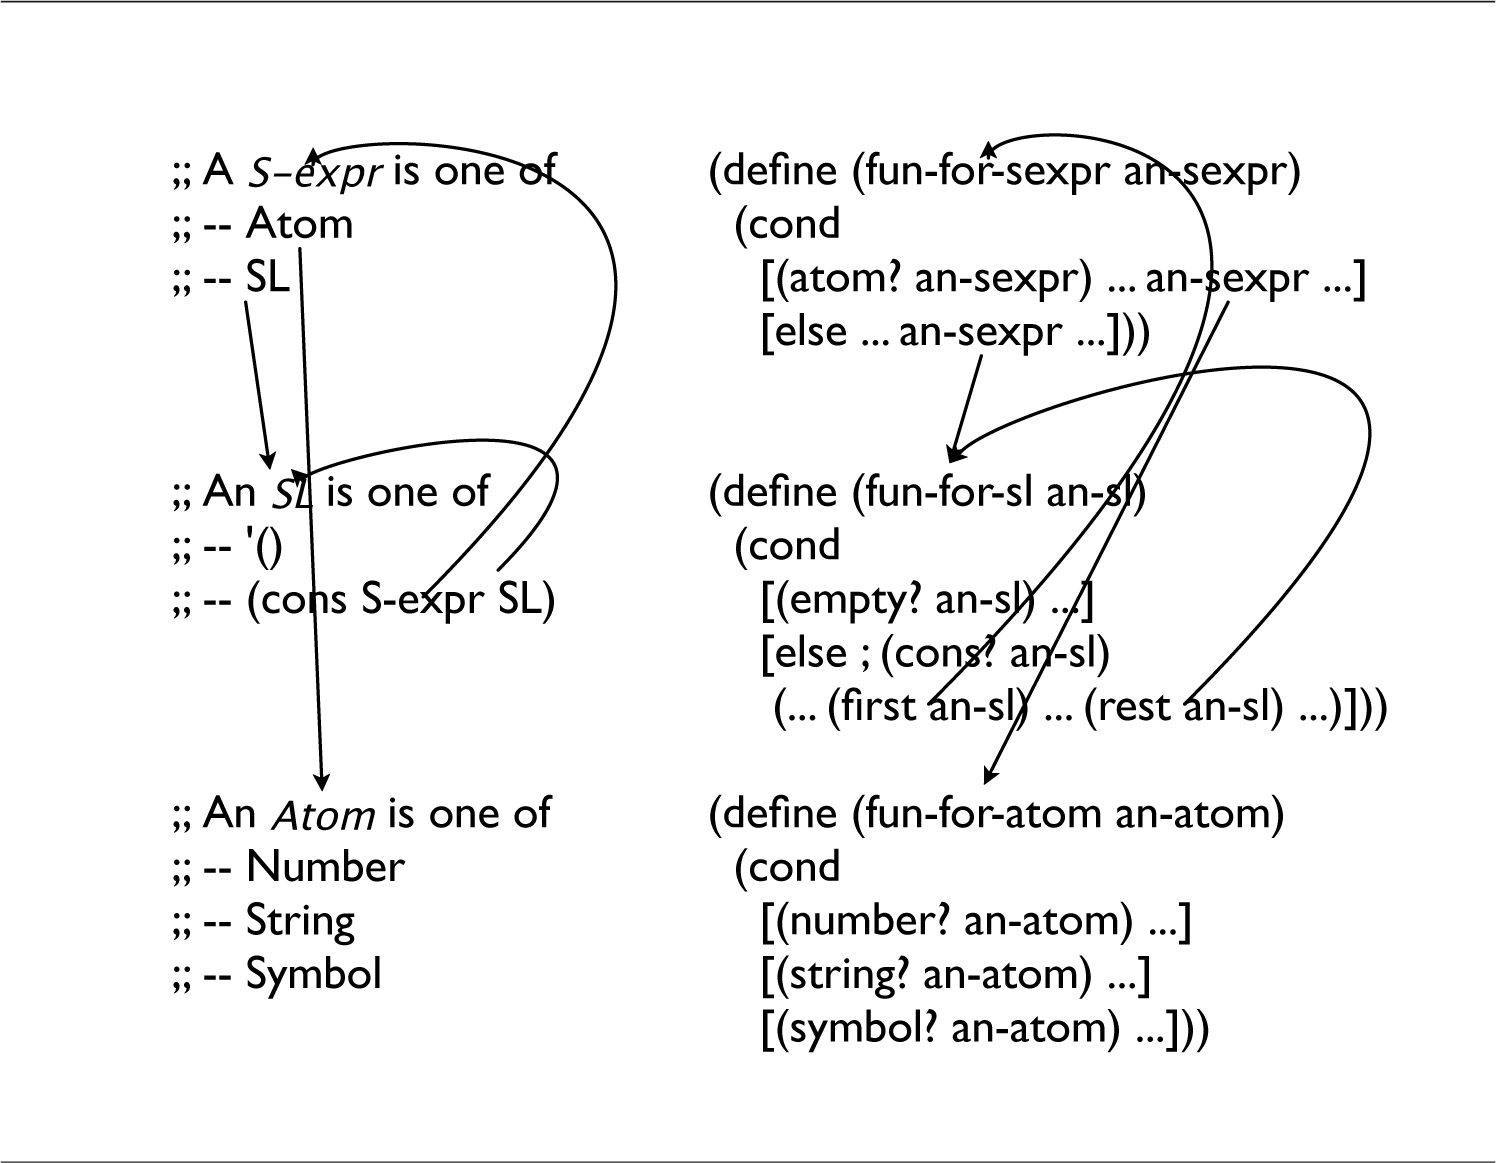
\includegraphics[width=0.85\textwidth]{images/00472.png}
  \caption{数据定义与模板间的引用关系对应 (Arrows for nests of data definitions and templates)}
  \label{fig:118}
\end{figure}

\begin{recipebox}[交织数据与相互递归函数的设计配方]
\textbf{1. 数据定义：} 当问题涉及多种不同形态的信息且相互嵌套时，编写一组互相引用的数据定义。画出各个定义之间的引用箭头（见图~\ref{fig:118} 左侧）。确保为每个定义都能构造出合法的基本用例。

\textbf{2. 签名与函数头：} 数据定义集合中有多少个数据定义，就\textbf{并行设计多少个函数}。每个函数专职处理其中一种数据定义，其余公共参数保持不变。

\textbf{3. 功能示例：} 构造测试用例，确保覆盖各定义之间的所有相互引用路径。

\textbf{4. 模板设计：} 为每个函数依据其主要输入的数据定义设计模板。数据定义中每出现一个指向其他定义的箭头，模板中就对应画出一个函数调用箭头（见图~\ref{fig:118} 右侧）。最终将箭头替换为具体的函数调用。

\textbf{5. 填充函数体：} 首先解决基准情形（不含递归或跨函数调用的分支），然后处理自引用和相互递归分支。

\textbf{6. 测试与排错：} 运行测试。若某个辅助函数存在缺陷，可能会同时引发主函数与辅助函数的报错。修复该辅助函数即可同时解决两处故障。
\end{recipebox}
